
%\frame[plain]{\titlepage}


%\end{frame}
{ % all template changes are local to this group.
    \setbeamertemplate{navigation symbols}{}
    \begin{frame}[plain]
        \begin{tikzpicture}[remember picture,overlay]
            \node[at=(current page.center)] {
                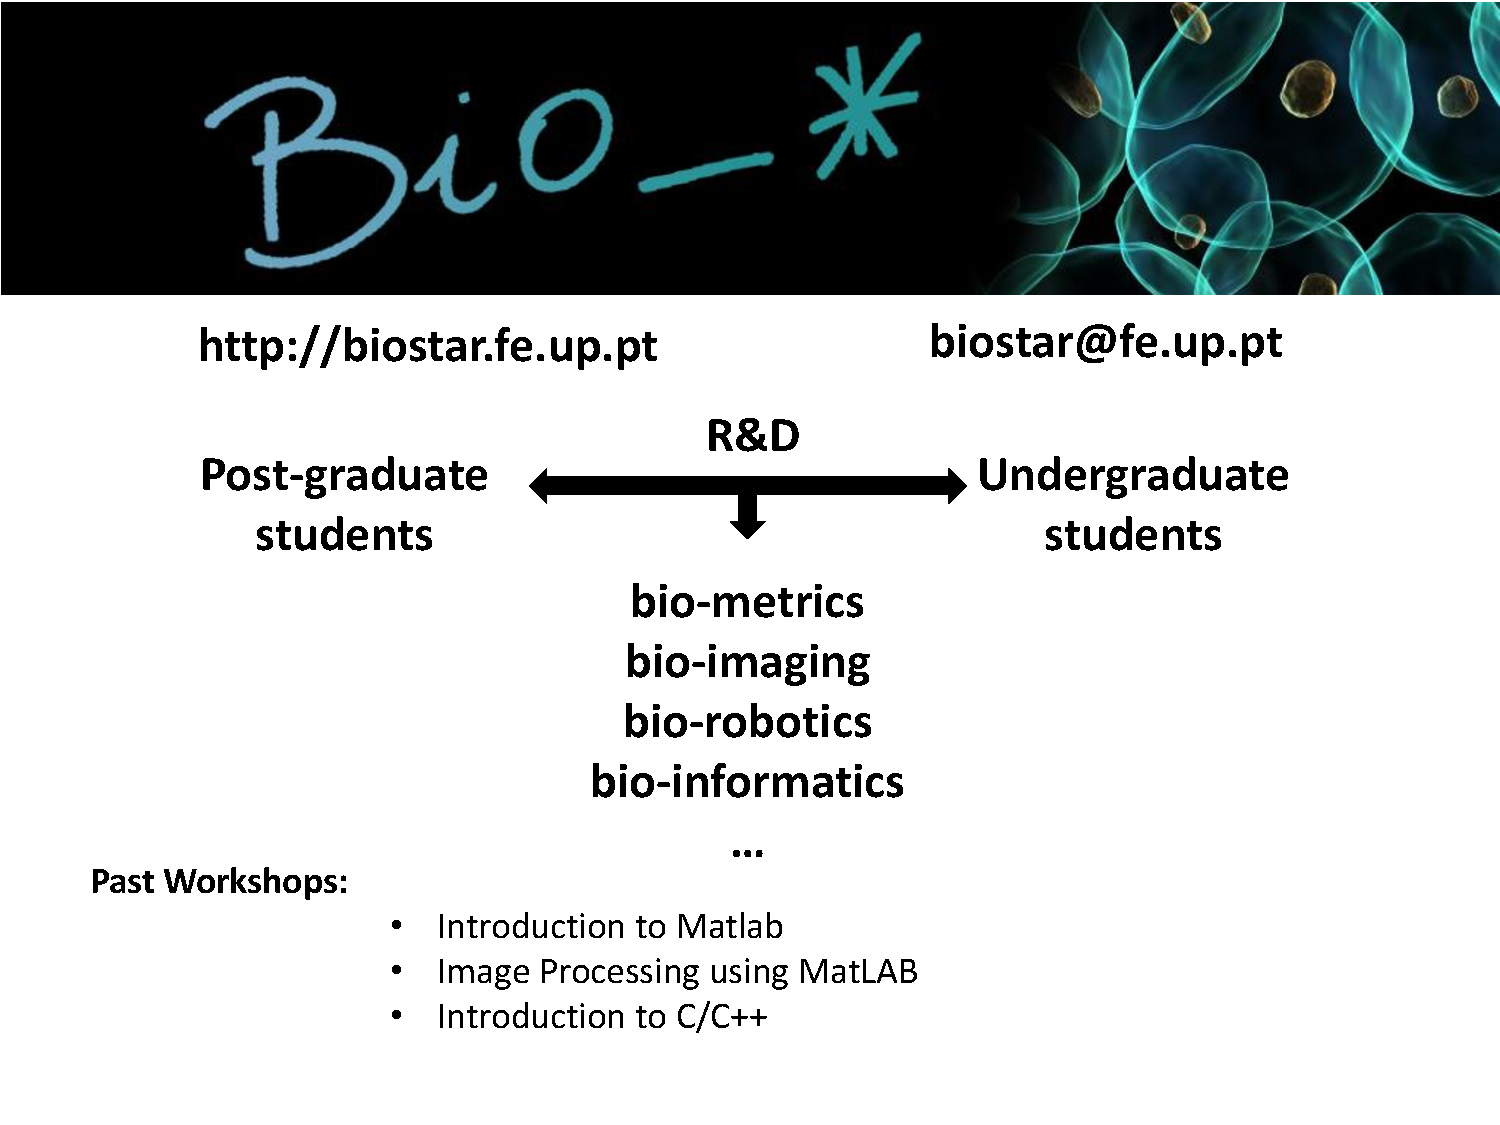
\includegraphics[width=\paperwidth]{slide_BioStar.pdf}
            };
        \end{tikzpicture}
     \end{frame}
}

\section*{Outline.}
\begin{frame}{Outline.}
\tableofcontents
\end{frame}

\AtBeginSubsection[]
{
 \begin{frame}<beamer>{Outline.}
   \tableofcontents[currentsection,currentsubsection]
 \end{frame}
}

%\begin{frame}{erro_propositado}
%erro propositado
%\end{frame}

\section{Introduction}

\subsection{Concepts}
\begin{frame}{What is \LaTeX{}?}
\begin{itemize}
\item \LaTeX{} is a typesetting system;
\item Allows the production of scientific (and non-scientific) documents;
\item High-quality results.
\end{itemize}
\small $\phantom{}^\star$Check references of this presentation for further information.
\end{frame}

\begin{frame}[fragile]{\LaTeX{} in a nutshell.}
Save following lines in a file named: minimal.tex
\begin{verbatim}
\documentclass{article}
\begin{document}
Small is beautiful.
\end{document}
\end{verbatim}
and then, on the command line (run twice at least):
\begin{verbatim}
$ pdflatex minimal
...
$ pdflatex minimal
\end{verbatim}
\end{frame}

\subsection{Installation}
\begin{frame}{Installing \LaTeX{}.}
\only<1>{\begin{figure}[!h]\centering\caption{MiKTeX homepage.}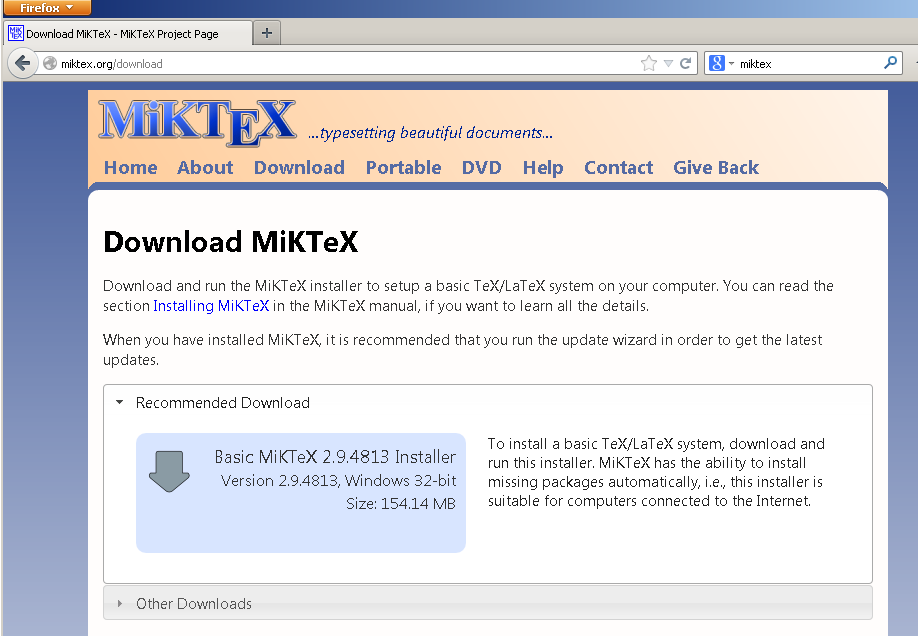
\includegraphics[width=0.65\textwidth]{installimgs/001.png}\end{figure}}
\only<2>{\begin{figure}[!h]\centering\caption{MiKTeX conditions.}
\includegraphics[width=0.6\textwidth]{installimgs/002.png}\end{figure}}
\only<3>{\begin{figure}[!h]\centering\caption{Standard configuration access profile.}
\includegraphics[width=0.6\textwidth]{installimgs/003.png}\end{figure}}
\only<4>{\begin{figure}[!h]\centering\caption{Installation directory.}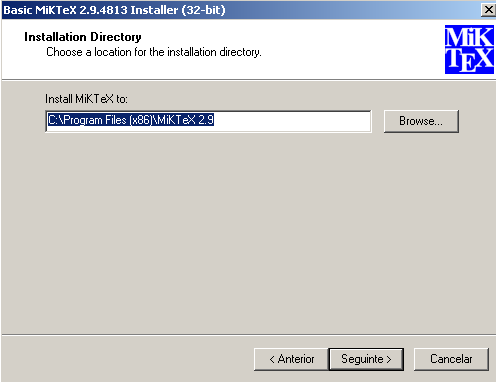
\includegraphics[width=0.6\textwidth]{installimgs/004.png}\end{figure}}
\only<5>{\begin{figure}[!h]\centering\caption{Some customizations (can be changed afterwards).}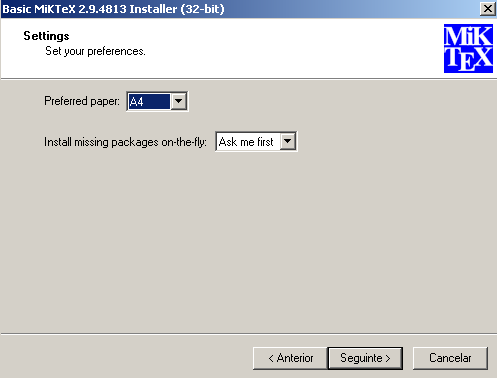
\includegraphics[width=0.5\textwidth]{installimgs/005.png}\end{figure}}
\only<6>{\begin{figure}[!h]\centering\caption{Review installation settings.}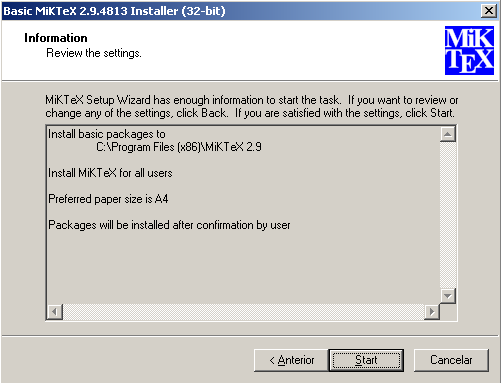
\includegraphics[width=0.65\textwidth]{installimgs/006.png}\end{figure}}
\only<7>{\begin{figure}[!h]\centering\caption{Installation (this may take a while).}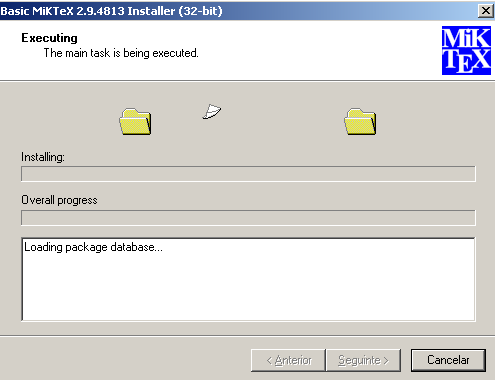
\includegraphics[width=0.65\textwidth]{installimgs/007.png}\end{figure}}
\only<8>{\begin{figure}[!h]\centering\caption{Installation (finished).}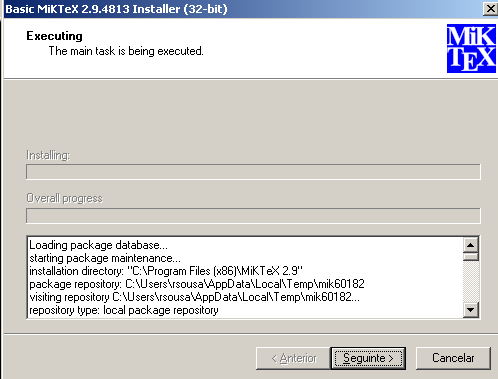
\includegraphics[width=0.65\textwidth]{installimgs/008.png}\end{figure}}
\only<9>{\begin{figure}[!h]\centering\caption{Installation finished.}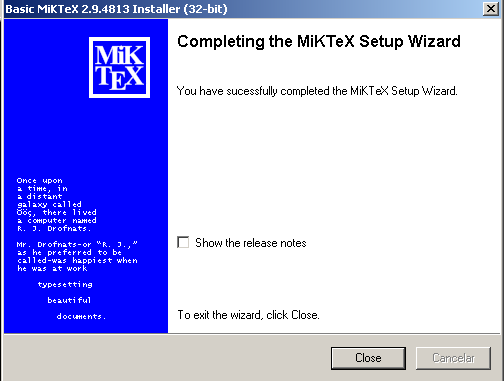
\includegraphics[width=0.65\textwidth]{installimgs/009.png}\end{figure}}
\end{frame}

\begin{frame}{Installing MiKTeX Portable.}
\only<1>{\begin{figure}[!h]\centering\caption{MiKTeX Portable Homepage.}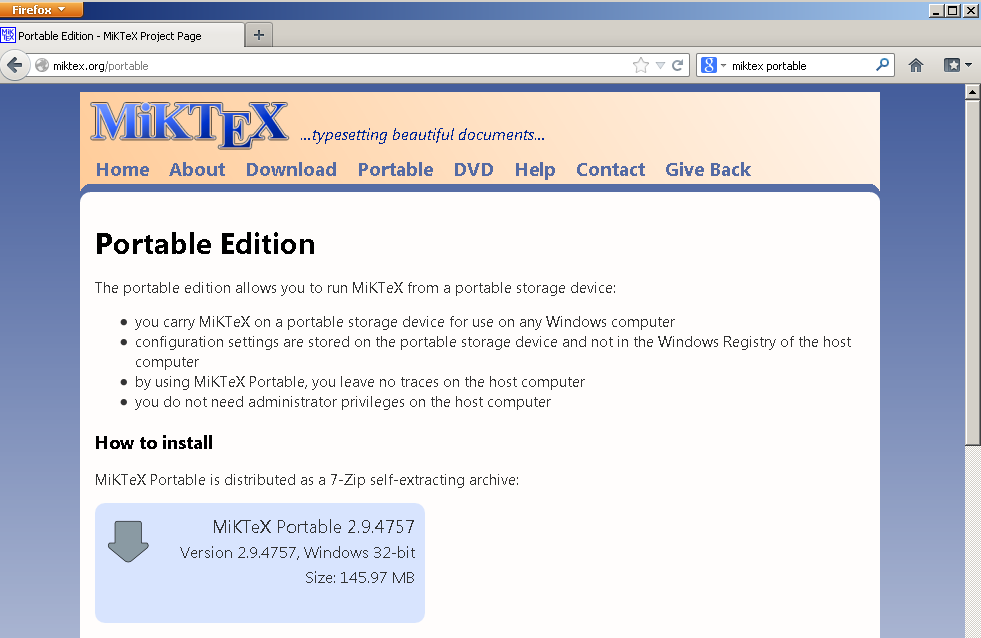
\includegraphics[width=0.5\textwidth]{installimgs/027.png}\end{figure}}
\only<2>{\begin{figure}[!h]\centering\caption{Extract to a given directory (e.g., pen drive).}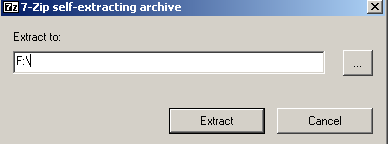
\includegraphics[width=0.5\textwidth]{installimgs/028.png}\end{figure}}
\only<3>{\begin{figure}[!h]\centering\caption{Extraction (this may take a while).}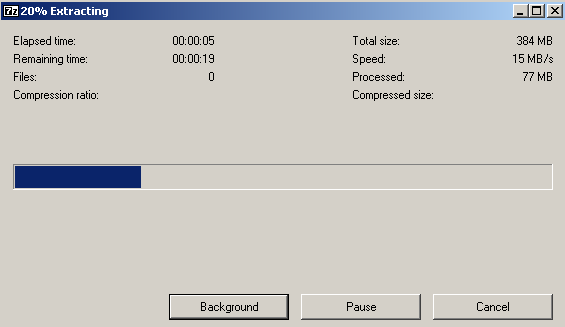
\includegraphics[width=0.5\textwidth]{installimgs/029.png}\end{figure}}
\only<4>{\begin{figure}[!h]\centering\caption{MiKTeX.}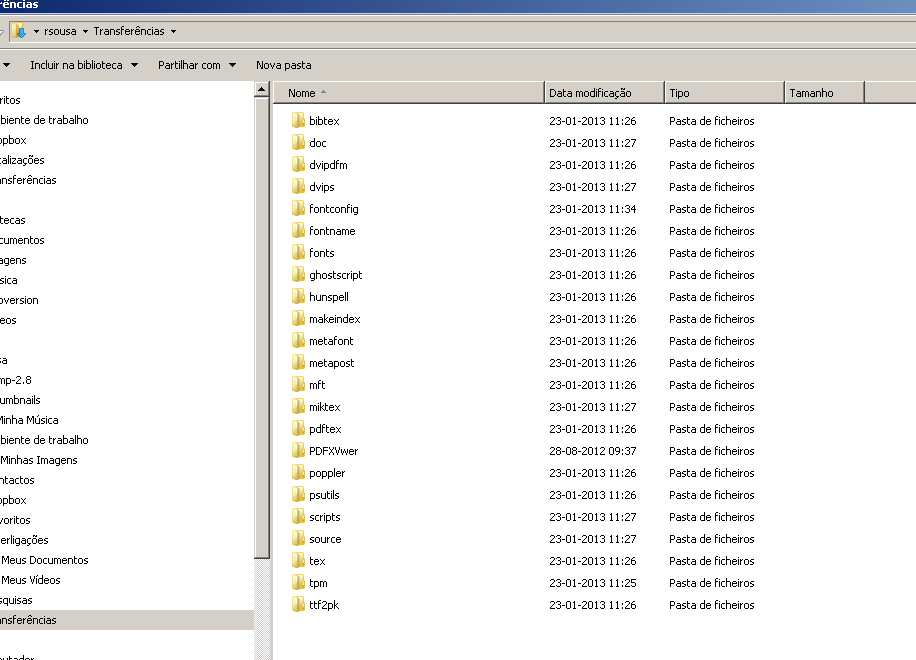
\includegraphics[width=0.5\textwidth]{installimgs/030.png}\end{figure}}
\end{frame}

\subsection{Maintenance}
\begin{frame}{Maintaining \LaTeX{} Updated - Part I.}
\only<1>{\begin{figure}[!h]\centering\caption{Maintaining \LaTeX{} (MiKTeX Portable).}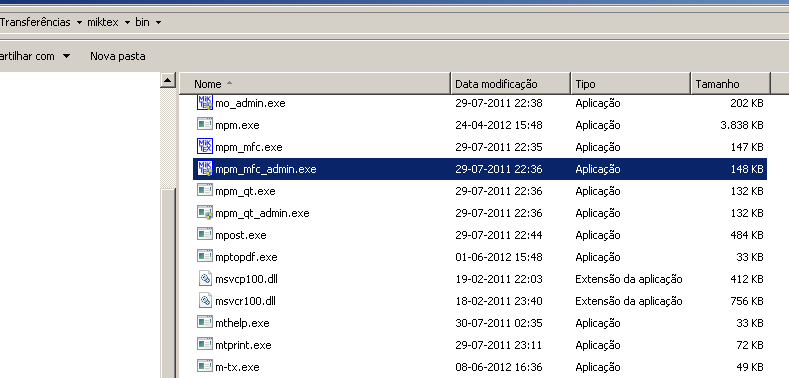
\includegraphics[width=0.7\textwidth]{installimgs/031.png}\end{figure}}
\only<2>{\begin{figure}[!h]\centering\caption{MiKTeX maintenance options (select update).}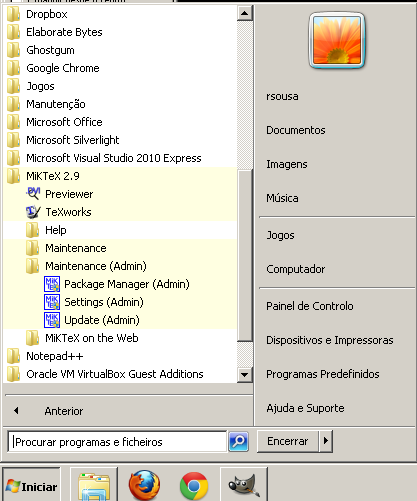
\includegraphics[width=0.5\textwidth]{installimgs/010.png}\end{figure}}
\only<3>{\begin{figure}[!h]\centering\caption{Select updates sources.}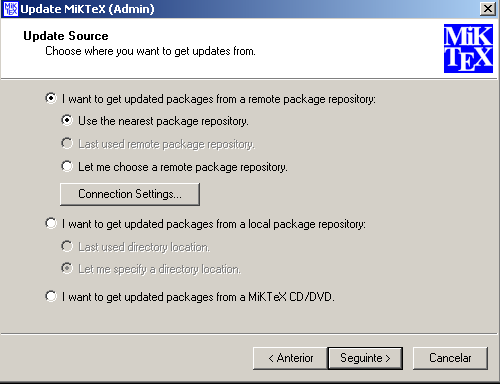
\includegraphics[width=0.6\textwidth]{installimgs/011.png}\end{figure}}
\only<4>{\begin{figure}[!h]\centering\caption{Example of packages to be updated.}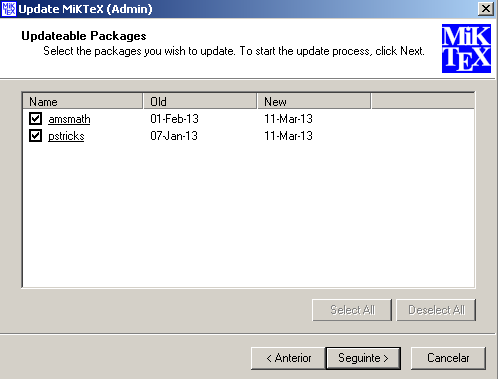
\includegraphics[width=0.6\textwidth]{installimgs/012.png}\end{figure}}
\only<5>{\begin{figure}[!h]\centering\caption{Update ongoing.}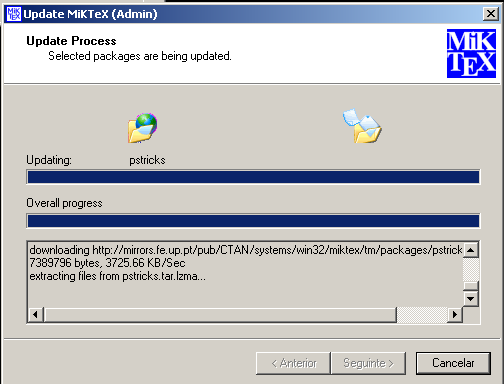
\includegraphics[width=0.65\textwidth]{installimgs/013.png}\end{figure}}
\only<6>{\begin{figure}[!h]\centering\caption{Update conclusion.}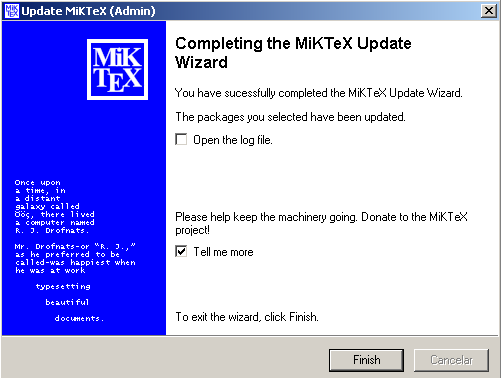
\includegraphics[width=0.65\textwidth]{installimgs/014.png}\end{figure}}
\end{frame}

\begin{frame}{Maintaining \LaTeX{} Updated - Part II.}
\only<1>{\begin{figure}[!h]\centering\caption{MiKTeX maintenance options (select package manager).}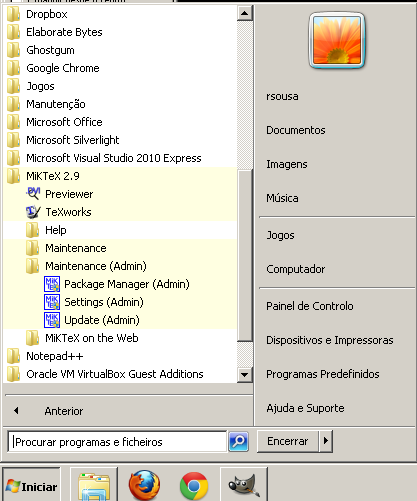
\includegraphics[width=0.5\textwidth]{installimgs/010.png}\end{figure}}
\only<2>{\begin{figure}[!h]\centering\caption{Packages listing.}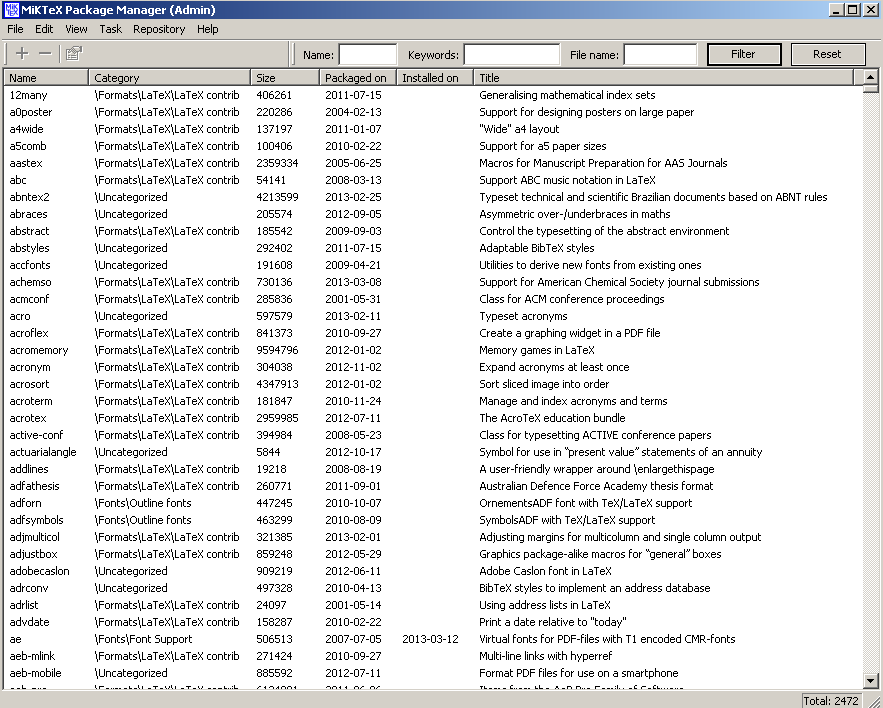
\includegraphics[width=0.5\textwidth]{installimgs/015.png}\end{figure}}
\only<3>{\begin{figure}[!h]\centering\caption{Search for ``ieee'' package.}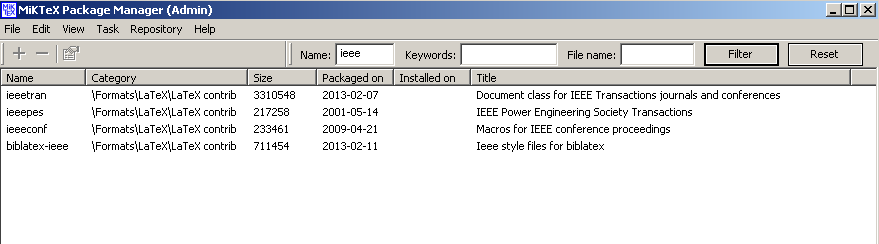
\includegraphics[width=0.8\textwidth]{installimgs/016.png}\end{figure}}
\only<4>{\begin{figure}[!h]\centering\caption{You can install by clicking in the ``+'' sign.}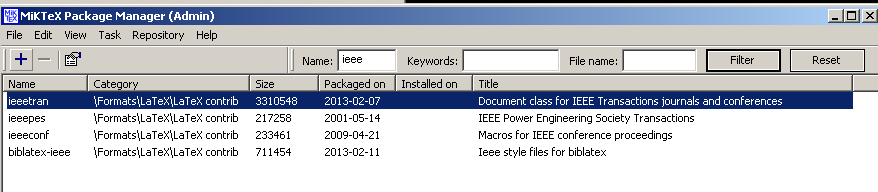
\includegraphics[width=0.8\textwidth]{installimgs/017.png}\end{figure}}
\only<5>{\begin{figure}[!h]\centering\caption{Or by pressing the right mouse button.}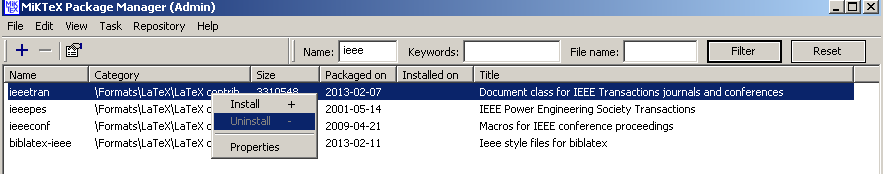
\includegraphics[width=0.8\textwidth]{installimgs/018.png}\end{figure}}
\only<6>{\begin{figure}[!h]\centering\caption{Package description.}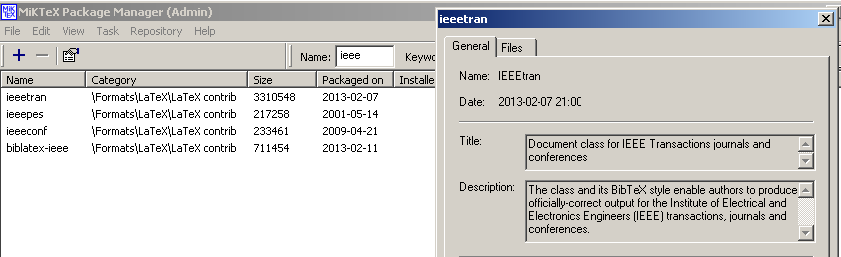
\includegraphics[width=0.65\textwidth]{installimgs/019.png}\end{figure}}
\only<7>{\begin{figure}[!h]\centering\caption{Installation confirmation box.}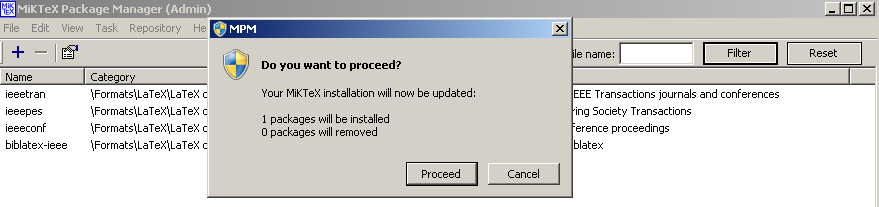
\includegraphics[width=0.8\textwidth]{installimgs/020.png}\end{figure}}
\only<8>{\begin{figure}[!h]\centering\caption{Installation.}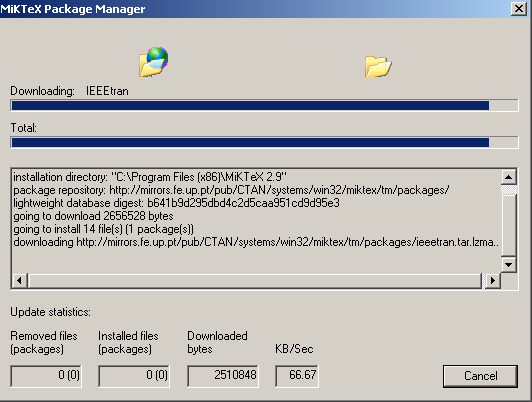
\includegraphics[width=0.6\textwidth]{installimgs/021.png}\end{figure}}
\only<9>{\begin{figure}[!h]\centering\caption{Changing package repository.}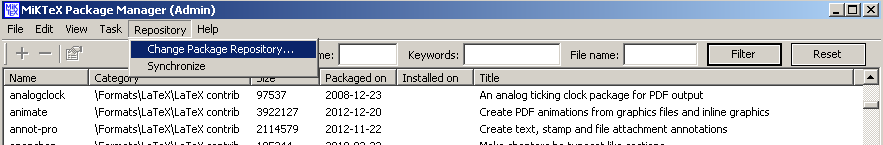
\includegraphics[width=0.8\textwidth]{installimgs/022.png}\end{figure}}
\only<10>{\begin{figure}[!h]\centering\caption{Select installation from internet for the most up to date packages.}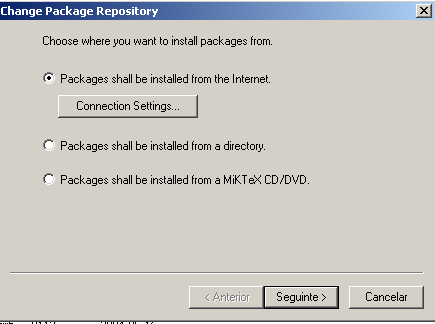
\includegraphics[width=0.65\textwidth]{installimgs/023.png}\end{figure}}
\only<11>{\begin{figure}[!h]\centering\caption{Select the closest one.}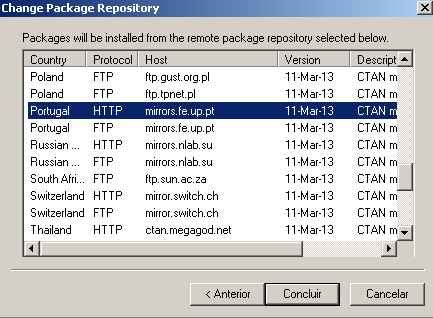
\includegraphics[width=0.65\textwidth]{installimgs/024.png}\end{figure}}
\only<12>{\begin{figure}[!h]\centering\caption{And let it synchronize.}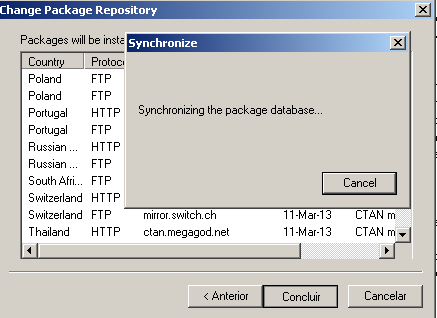
\includegraphics[width=0.65\textwidth]{installimgs/025.png}\end{figure}}
\end{frame}


\begin{frame}{Maintaining \LaTeX{} Updated - Part III.}
\only<1>{\begin{figure}[!h]\centering\caption{MiKTeX maintenance options (select package manager).}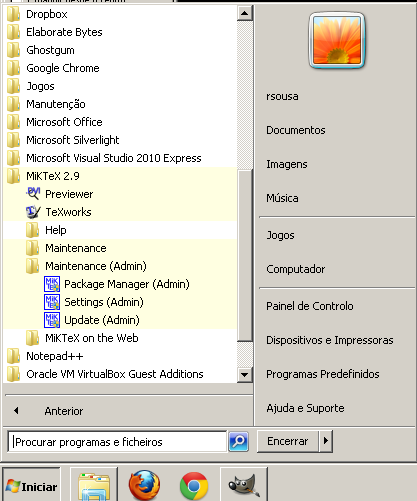
\includegraphics[width=0.5\textwidth]{installimgs/010.png}\end{figure}}
\only<2>{\begin{figure}[!h]\centering\caption{Change settings.}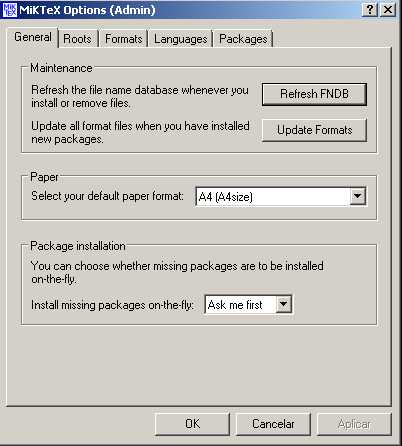
\includegraphics[width=0.5\textwidth]{installimgs/026.png}\end{figure}}
\end{frame}

\section{\LaTeX{} Documents}
\subsection{Graphical User Interface (GUI)}
\begin{frame}{User Interface: TeXworks}
\only<1>{\begin{figure}[!h]\centering\caption{Right click on the main \LaTeX{} file and press ``open with'' TeXworks.}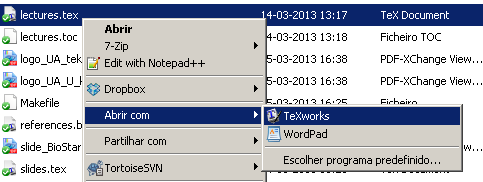
\includegraphics[width=0.5\textwidth]{imgsgui/001.png}\end{figure}}
\only<2>{\begin{figure}[!h]\centering\caption{Expected result (for this presentation).}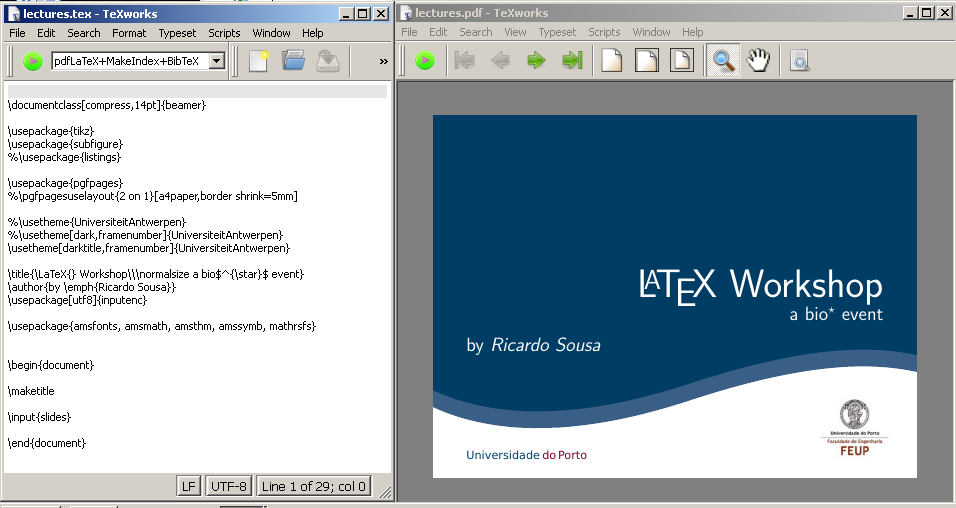
\includegraphics[width=0.7\textwidth]{imgsgui/002.png}\end{figure}}
\only<3>{\begin{figure}[!h]\centering\caption{Syntax highlight.}
\includegraphics[width=0.5\textwidth]{imgsgui/003.png}\end{figure}}
\only<4>{\begin{figure}[!h]\centering\caption{Expected result.}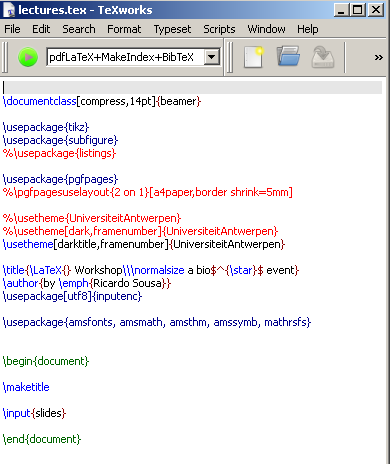
\includegraphics[width=0.5\textwidth]{imgsgui/004.png}\end{figure}}
\end{frame}

\begin{frame}{TeXworks: Compiling.}
\only<1>{\begin{figure}[!h]\centering\caption{Compiling.}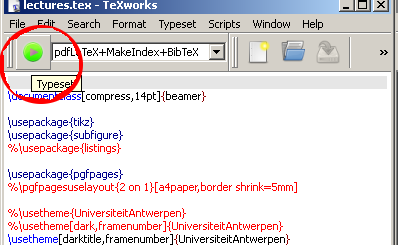
\includegraphics[width=0.5\textwidth]{imgsgui/005.png}\end{figure}}
\only<2>{\begin{figure}[!h]\centering\caption{Console output.}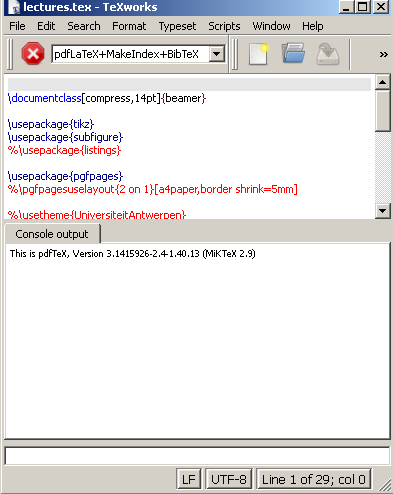
\includegraphics[width=0.5\textwidth]{imgsgui/006.png}\end{figure}}
\only<3>{\begin{figure}[!h]\centering\caption{Pop-up window to install missing packages.}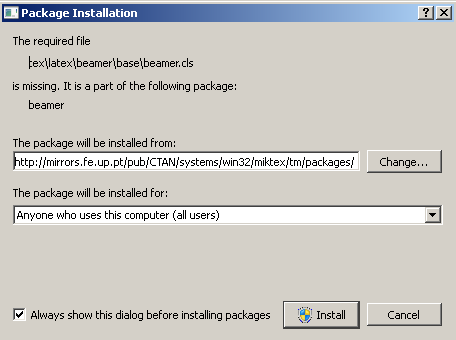
\includegraphics[width=0.5\textwidth]{imgsgui/007.png}\end{figure}}
\only<4>{\begin{figure}[!h]\centering\caption{Compilation unsuccessful.}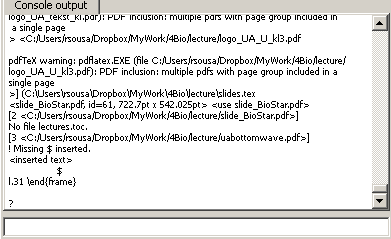
\includegraphics[width=0.5\textwidth]{imgsgui/013.png}\end{figure}}
\end{frame}

\begin{frame}{Command line compilation.}
\only<1>{\begin{figure}[!h]\centering\caption{Generating compile script.}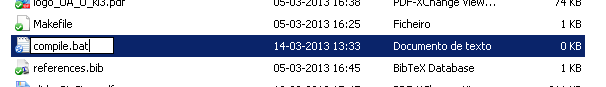
\includegraphics[width=0.7\textwidth]{imgsgui/008.png}\end{figure}}
\only<2>{\begin{figure}[!h]\centering\caption{3 main lines of code.}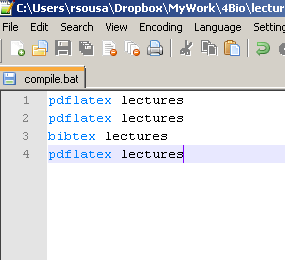
\includegraphics[width=0.5\textwidth]{imgsgui/009.png}\end{figure}}
\only<3>{\begin{figure}[!h]\centering\caption{Open a command line window}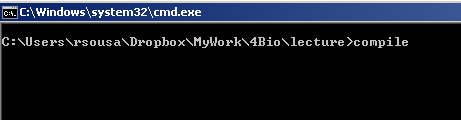
\includegraphics[width=0.5\textwidth]{imgsgui/010.png}\end{figure}}
\only<4>{\begin{figure}[!h]\centering\caption{Pop-up window to install missing packages.}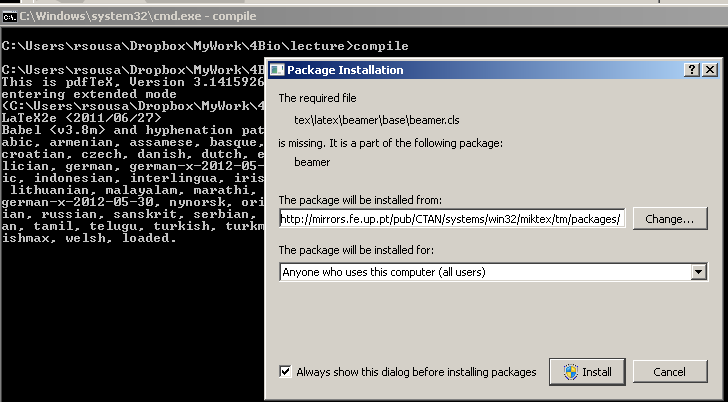
\includegraphics[width=0.5\textwidth]{imgsgui/011.png}\end{figure}}
\only<5>{\begin{figure}[!h]\centering\caption{Compilation successful.}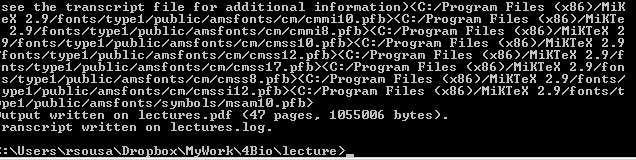
\includegraphics[width=0.5\textwidth]{imgsgui/012.png}\end{figure}}
\only<6>{\begin{figure}[!h]\centering\caption{Compilation unsuccessful.}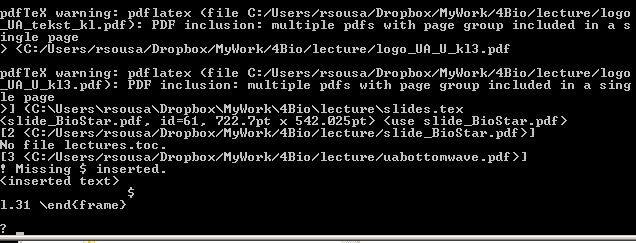
\includegraphics[width=0.5\textwidth]{imgsgui/014.png}\end{figure}}
\only<7>{\begin{figure}[!h]\centering\caption{Good practice: erase those auxiliary files.}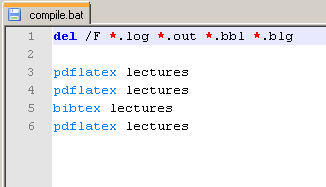
\includegraphics[width=0.5\textwidth]{imgsgui/015.png}\end{figure}}
\end{frame}



\subsection{Creating Documents with \LaTeX{}}
\begin{frame}[fragile]{Creating my first \LaTeX{} Manuscript}
\begin{verbatim}
\documentclass{article}
% preamble
\begin{document}
% core
\end{document}
\end{verbatim}
\end{frame}


\begin{frame}[fragile]{Creating my first \LaTeX{} Manuscript}
Typical structure:
\footnotesize
\begin{verbatim}
\documentclass[twoside,a4paper,10pt]{article}
% preamble
\begin{document}
% core
\end{document}
\end{verbatim}
\end{frame}

\begin{frame}[fragile]{Creating my first \LaTeX{} Manuscript}
An a4 paper with font size of 10 points:
\footnotesize
\begin{verbatim}
\documentclass[twoside,a4paper,10pt]{article}
% preamble
\usepackage[utf8]{inputenc} % general input encondings
\begin{document}
% core
\end{document}
\end{verbatim}
\end{frame}

\begin{frame}[fragile]{Creating my first \LaTeX{} Manuscript}
Portuguese support:
\footnotesize
\begin{verbatim}
\documentclass[twoside,a4paper,10pt]{article}
% preamble
\usepackage[utf8]{inputenc} % general input encondings
\usepackage[portuguese]{babel}
\begin{document}
% core
\end{document}
\end{verbatim}
\end{frame}

\begin{frame}[fragile]{Creating my first \LaTeX{} Manuscript}
Different packages at your disposal:
\footnotesize
\begin{enumerate}
\item \verb1\usepackage{graphicx}1: figures;
\item \verb1\usepackage{subfig}1: when working with multiple figures;
\item \verb1\usepackage{cite}1: citations;
\item \verb1\usepackage{amsmath}1: mathematical features;
\item \verb1\usepackage{amssymb}1: mathematical symbols;
\item and lots more $\ldots$
\end{enumerate}
Check \url{http://www.ctan.org}.
\end{frame}


\begin{frame}[fragile]{Creating my first \LaTeX{} Manuscript}
Creating Lists:

The itemize environment is for simple lists, the enumerate environment for enumerated lists, and the description environment for descriptions.
\end{frame}

\begin{frame}[fragile]{Creating my first \LaTeX{} Manuscript}
Follows some examples:
\scriptsize
\begin{verbatim}
\begin{enumerate}
\item You can mix the list environments to your taste:
  \begin{itemize}
   \item But it might start to look silly.
   \item[-] With a dash.
 \end{itemize}
\item Therefore remember:
\begin{description}
   \item[Stupid] things will not become smart because they are in a list.
   \item[Smart] things, though, can be presented beautifully in a list.
\end{description}
\end{enumerate}
\end{verbatim}
\end{frame}

\begin{frame}[fragile]{Creating my first \LaTeX{} Manuscript}
Including a figure:
\footnotesize
\begin{verbatim}
\documentclass[twoside,a4paper,10pt]{article}
% preamble
\usepackage[utf8]{inputenc} % general input encondings
\usepackage{graphicx}

\begin{document}
\begin{figure}
  
\includegraphics{img.pdf}
\end{figure}
\end{document}
\end{verbatim}
\end{frame}

\begin{frame}[fragile]{Creating my first \LaTeX{} Manuscript}
\begin{columns}[c]
\column{1.5in}
\begin{verbatim}
{\tiny A}
{\scriptsize A}
{\footnotesize A}
{\small A}
{\normalsize A}
{\large A}
{\Large A}
{\LARGE A}
{\huge A}
{\Huge A}
\end{verbatim}
\column{2.5in}
{\tiny A}
{\scriptsize A}
{\footnotesize A}
{\small A}
{\normalsize A}
{\large A}
{\Large A}
{\LARGE A}
{\huge A}
{\Huge A}
%\framebox{\includegraphics[width=1.5in]{p2005}}
\end{columns}
\end{frame}


\begin{frame}[fragile]{Creating my first \LaTeX{} Manuscript}
Including a figure:
\footnotesize
\begin{verbatim}
\documentclass[twoside,a4paper,10pt]{article}
% preamble
\usepackage[utf8]{inputenc} % general input encondings
\usepackage{graphicx}
\begin{document}

Logo.
\begin{figure}
  \includegraphics{img.pdf}
\end{figure}
End of document.
\end{document}
\end{verbatim}
\end{frame}

\begin{frame}[fragile]{Creating my first \LaTeX{} Manuscript}
Including a figure (Can you find the difference?):
\footnotesize
\begin{verbatim}
\documentclass[twoside,a4paper,10pt]{article}
% preamble
\usepackage[utf8]{inputenc} % general input encondings
\usepackage{graphicx}
\begin{document}

Logo.
\begin{figure}[!h]
  \includegraphics{img.pdf}
\end{figure}
End of document.
\end{document}
\end{verbatim}
\end{frame}

\begin{frame}[fragile]{Creating my first \LaTeX{} Manuscript}
Including a figure (Can you find the difference?):
\footnotesize
\begin{verbatim}
\documentclass[twoside,a4paper,10pt]{article}
% preamble
\usepackage[utf8]{inputenc} % general input encondings
\usepackage{graphicx}
\begin{document}

Logo.
\begin{figure}[!h] % <-------------- LOOK!!
  \includegraphics{img.pdf}
\end{figure}
End of document.
\end{document}
\end{verbatim}
\end{frame}


\begin{frame}{Floating Bodies.}
How it affects the document?
\begin{itemize}
\item to place a figure/table right here (h);
\item or at the bottom (b) of some page;
\item or on a special floats page (p);
\item and, all this even if it does not look that good (!)
\item if no placement specifier is given: [tbp]
\end{itemize}
\end{frame}

\begin{frame}[fragile]{Creating my first \LaTeX{} Manuscript}
To include figure between two paragraphs:
\footnotesize
\begin{verbatim}
\documentclass[twoside,a4paper,10pt]{article}
% preamble
\usepackage[utf8]{inputenc} % general input encondings
\usepackage{graphicx}
\begin{document}

Logo.
\begin{figure}[!h] 
  \includegraphics{img.pdf}
\end{figure}

End of document.
\end{document}
\end{verbatim}
\end{frame}


\begin{frame}[fragile]{Creating my first \LaTeX{} Manuscript}
Can we change the image size? Yes!
\footnotesize
\begin{verbatim}
\documentclass[twoside,a4paper,10pt]{article}
% preamble
\usepackage[utf8]{inputenc} % general input encondings
\usepackage{graphicx}
\begin{document}

Logo.
\begin{figure}[!h] 
  \includegraphics[width=0.5\textwidth]{img.pdf}
\end{figure}

End of document.
\end{document}
\end{verbatim}
\end{frame}

\begin{frame}[fragile]{Creating my first \LaTeX{} Manuscript}
Can we center the image? Of course!
\footnotesize
\begin{verbatim}
\documentclass[twoside,a4paper,10pt]{article}
% preamble
\usepackage[utf8]{inputenc} % general input encondings
\usepackage{graphicx}
\begin{document}

Logo.
\begin{figure}[!h] 
  \centering
  \includegraphics[width=0.5\textwidth]{img.pdf}
\end{figure}

End of document.
\end{document}
\end{verbatim}
\end{frame}

\begin{frame}[fragile]{Creating my first \LaTeX{} Manuscript}
Can we center the image? Another way!
\footnotesize
\begin{verbatim}
\documentclass[twoside,a4paper,10pt]{article}
% preamble
\usepackage[utf8]{inputenc} % general input encondings
\usepackage{graphicx}
\begin{document}

Logo.
\begin{figure}[!h] 
  \begin{center}
  \includegraphics[width=0.5\textwidth]{img.pdf}
  \end{center}
\end{figure}

End of document.
\end{document}
\end{verbatim}
\end{frame}

\begin{frame}[fragile]{Creating my first \LaTeX{} Manuscript}
And what about captions? Easy stuff :)
\footnotesize
\begin{verbatim}
\begin{figure}[!h] 
  \centering                  
  \includegraphics[width=0.5\textwidth]{img.pdf}
  \caption{Faculty Logo.}
\end{figure}
\end{verbatim}
\end{frame}

\begin{frame}[fragile]{Creating my first \LaTeX{} Manuscript}
Including more than one figure.
\footnotesize
\begin{verbatim}
\begin{figure}[!h] 
  \centering                  
  \includegraphics[width=0.5\textwidth]{img.pdf}
  \includegraphics[width=0.5\textwidth]{img.pdf}
  \caption{Faculty Logo.}
\end{figure}
\end{verbatim}
\end{frame}


\begin{frame}[fragile]{Creating my first \LaTeX{} Manuscript}
However, we should use package `subfig' which provides support for the inclusion of small, ‘sub’, figures and tables.
\scriptsize
\begin{verbatim}
...
\usepackage{subfig}
\begin{document}
...
\begin{figure}[!h]
\subfloat[Imagem 1.]{\includegraphics[width=0.5\textwidth]{img.pdf}}
\subfloat[Imagem 2.]{\includegraphics[width=0.5\textwidth]{img.pdf}}
\end{figure}
\end{verbatim}
\end{frame}


\begin{frame}[fragile]{Creating my first \LaTeX{} Manuscript}
How to create tables? The simplest way is:
\footnotesize
\begin{verbatim}
\begin{tabular}{ccc}
Evolutionary & SA & Simulated Annealing \\ 
\end{tabular}
\end{verbatim}
\begin{itemize}
\item \emph{tabular} is the environment for tables;
\item Triple ``c'' for three columns with centered (c) text;
\item ``\&'' is the column separator;
\item $\backslash\backslash$  is the new line;
\end{itemize}
\end{frame}


\begin{frame}[fragile]{Creating my first \LaTeX{} Manuscript}
How to create tables? The simplest way is:
\footnotesize
\begin{verbatim}
\begin{tabular}{|p{3cm}|c|c|}
Evolutionary & SA & Simulated Annealing \\ 
\end{tabular}
\end{verbatim}
\begin{itemize}
\item besides ``c'' we can have:
      \begin{itemize}
        \item \verb!l!: left;
        \item \verb!r!: right;
        \item \verb!p{2cm}!: paragraph with 2cm width.
      \end{itemize}
\item we can also stylish our table by putting bars \verb!|.|!
\end{itemize}
\end{frame}


\begin{frame}[fragile]{Creating my first \LaTeX{} Manuscript}
How to create tables? The simplest way is:
\footnotesize
\begin{verbatim}
\begin{tabular}{|p{3cm}|c|c|}
\hline
Evolutionary & ZO & Genetic Algorithm\\ 
Evolutionary & SA & Simulated Annealing \\ 
\hline
\end{tabular}
\end{verbatim}
adding horizontal lines with \verb!\hline!
\end{frame}


\begin{frame}[fragile]{Creating my first \LaTeX{} Manuscript}
Merging cells (rows).
\footnotesize
\begin{verbatim}
\usepackage{multirow}
...
\begin{document}
\begin{tabular}{|p{3cm}|c|c|}
\hline
\multirow{2}{*}{Evolutionary} & ZO & Genetic Algorithm\\ 
                              & SA & Simulated Annealing \\ 
\hline
\end{tabular}
...
\end{document}
\end{verbatim}
\end{frame}


\begin{frame}[fragile]{Creating my first \LaTeX{} Manuscript}
Merging cells (columns).
\footnotesize
\begin{verbatim}
\begin{tabular}{|p{3cm}|c|c|}
\hline
\multicolumn{3}{|c|}{Heuristic Algorithms} \\
\hline
\multirow{2}{*}{Evolutionary} & ZO & Genetic Algorithm\\ 
                              & SA & Simulated Annealing \\ 
\hline
\end{tabular}
\end{verbatim}
\end{frame}

\begin{frame}[fragile]{Creating my first \LaTeX{} Manuscript}
\footnotesize
\begin{verbatim}
\begin{table}[!t]
\begin{tabular}{|p{3cm}|c|c|}
\hline
\multicolumn{3}{|c|}{Heuristic Algorithms} \\
\hline
\multirow{2}{*}{Evolutionary} & ZO & Genetic Algorithm\\ 
                              & SA & Simulated Annealing \\ 
\hline
\end{tabular}
\caption{Table of some Heuristic Algorithms.}
\end{table}
\end{verbatim}
\end{frame}


\begin{frame}[fragile]{Creating my first \LaTeX{} Manuscript}
How can we reference tables in the document?
\footnotesize
\begin{verbatim}
\begin{table}[!t]
\begin{tabular}{|p{3cm}|c|c|}
\hline
\multicolumn{3}{|c|}{Heuristic Algorithms} \\
\hline
\multirow{2}{*}{Evolutionary} & ZO & Genetic Algorithm\\ 
                              & SA & Simulated Annealing \\ 
\hline
\end{tabular}
\caption{Table of some Heuristic Algorithms.}
\label{tab:table}
\end{table}
Please check Table~\ref{tab:table}.
\end{verbatim}
\end{frame}

\begin{frame}[fragile]{Creating my first \LaTeX{} Manuscript}
Can I divide my document by sections? Of course
\footnotesize
\begin{verbatim}
\section{Introduction}
...
\section{State-of-the-Art}
\subsection{Biology Concepts}
...
\subsection{Image Processing}
...
\subsection{Pattern Recognition}
...
\end{verbatim}
\end{frame}

\begin{frame}[fragile]{Creating my first \LaTeX{} Manuscript}
References can be used anywhere. 
\scriptsize
\begin{verbatim}
\section{Introduction}
\label{sec:intro}
...
\section{State-of-the-Art}
\label{sec:soa}
\subsection{Biology Concepts}
\label{sec:bio}
...
\subsection{Image Processing}
\label{sec:ip}
...
\subsection{Pattern Recognition}
\label{sec:pr}
...

Further image processing details can be found in Section~\ref{sec:ip}.
\end{verbatim}
\end{frame}

\begin{frame}[fragile]{Creating my first \LaTeX{} Manuscript}
Document can also be divided in parts, chapters and so on. 
\scriptsize
\begin{verbatim}
\documentclass[twoside,a4paper,10pt]{book}
...
\begin{document}
\part{Basic Concepts: Part I}
\chapter{Beginning}
\section{How does it starts?}

\part{Basic Concepts: Part II}
\end{document}
\end{verbatim}
\end{frame}

\begin{frame}[fragile]{Creating my first \LaTeX{} Manuscript}
Title, authors..
\scriptsize
\begin{verbatim}
\documentclass[twoside,a4paper,10pt]{book}
% preamble
\usepackage[utf8]{inputenc} % general input encondings
\usepackage{graphicx}
\usepackage{multirow}

\title{Book Sample}
\begin{document}
\tableofcontents % simple, isn't it?

\part{Basic Concepts: Part I}
\chapter{Beginning}
\section{How does it starts?}

\part{Basic Concepts: Part II}
\end{document}
\end{verbatim}
\end{frame}

\begin{frame}[fragile]{Creating my first \LaTeX{} Manuscript}
\emph{maketitle} after the \verb!\begin{document}!
\scriptsize
\begin{verbatim}
\documentclass[twoside,a4paper,10pt]{book}
% preamble
\usepackage[utf8]{inputenc} % general input encondings
\usepackage{graphicx}
\usepackage{multirow}

\title{Book Sample}
\begin{document}
\maketitle % tells latex to put title here!
\tableofcontents % simple, isn't it?

\part{Basic Concepts: Part I}
\chapter{Beginning}
\section{How does it starts?}

\part{Basic Concepts: Part II}
\end{document}
\end{verbatim}
\end{frame}

\begin{frame}[fragile]{Creating my first \LaTeX{} Manuscript}
author and date
\scriptsize
\begin{verbatim}
\title{Book Sample}
\author{X and Y}
\date{16/03/2013}
\begin{document}
\maketitle
\tableofcontents % simple, isn't it?
\end{verbatim}
\normalsize
It is also possible to specify current date through command \verb!\date{\today}!
\end{frame}


\begin{frame}[fragile]{Creating my first \LaTeX{} Manuscript}
Mathematical Formulas
\scriptsize
\begin{verbatim}
\begin{equation}
e = mc^2
\label{eq:massenergy}
\end{equation}
Mass Energy Einstein equivalence formula (Eq.~\ref{eq:massenergy}).
\end{verbatim}
\begin{itemize}
\item equation environment;
\item $\wedge$ is for superscript text.
\end{itemize}
\end{frame}


\begin{frame}[fragile]{Creating my first \LaTeX{} Manuscript}
Mathematical Formulas (summations):
\scriptsize
\begin{verbatim}
\begin{equation}
1/N \sum_{i=1}^N x_i
\end{equation}
\end{verbatim}
\begin{itemize}
\item $\vee$ is for subscript;
\item $/$ can be substituted by \verb!\frac{1}{N}! (output result will be different, $\frac{1}{N}$).
\end{itemize}
\end{frame}


\begin{frame}[fragile]{Creating my first \LaTeX{} Manuscript}
Symbols:
\begin{verbatim}
 \alpha  \theta      \tau          
 \beta   \vartheta   \pi     
 \gamma  \gamma      \varpi  
\end{verbatim}
You do not need know them by heart.
Check \url{http://www.tex.ac.uk/tex-archive/info/symbols/comprehensive/symbols-a4.pdf}
\end{frame}

\begin{frame}{Creating my first \LaTeX{} Manuscript}
Symbols:
\begin{align}
 \alpha & & \theta    &  & \tau\\
 \beta  & & \vartheta & & \pi \\   
 \gamma & & \gamma    & & \varpi
\end{align}
\end{frame}


\begin{frame}[fragile]{Creating my first \LaTeX{} Manuscript}
Mathematical Formulas (without numbering):
\scriptsize
\begin{verbatim}
\begin{equation*}
1/N \sum_{i=1}^N x_i
\label{eq:avg}
\end{equation*}
Average formula (Eq.~\ref{eq:avg}).
\end{verbatim}
\normalsize
What you think that will happen?
\pause
The $\star$ symbol can be also applied in tables, figures, sections, $\ldots$.
\end{frame}

\begin{frame}[fragile]{Creating my first \LaTeX{} Manuscript}
Mathematical Formulas (inline):
\scriptsize
\begin{verbatim}
$1/N \sum_{i=1}^N x_i$
\end{verbatim}
\normalsize
\pause
you can also put inline formulas centered in the text
\scriptsize
\begin{verbatim}
\[
1/N \sum_{i=1}^N x_i 
\]
\end{verbatim}
\end{frame}


\begin{frame}[fragile]{Creating my first \LaTeX{} Manuscript}
Finally, we also may need to add some bibliographic references.

Add \verb!bibtex! to the compilation script (TeXworks already does this!).
\scriptsize
\begin{verbatim}
pdflatex document
pdflatex document
bibtex document
pdflatex document
\end{verbatim}
\end{frame}

\begin{frame}[fragile]{Creating my first \LaTeX{} Manuscript}
You need to create a file for the references (named it references.bib) and the following content:
\scriptsize
\begin{verbatim}
book{calder1979einstein,                       % key
  title={Einstein's universe},                 % title
  author={Calder, Nigel and Albert, Einstein}, % author
  year={1979},                                 % year
  publisher={Viking Press}                     % publisher
}
\end{verbatim}
\end{frame}

\begin{frame}[fragile]{Creating my first \LaTeX{} Manuscript}
In your \LaTeX{} main file you should call now the bibliography file.
\scriptsize
\begin{verbatim}
\begin{document}

\begin{equation}
e = mc^2
\label{eq:massenergy}
\end{equation}
Mass Energy Einstein equivalence formula (Eq.~\ref{eq:massenergy}).

\bibliographystyle{plain}
\bibliography{references}

\end{document}
\end{verbatim}
\end{frame}

\begin{frame}[fragile]{Creating my first \LaTeX{} Manuscript}
Previous gave a warning when generating the references list. Do you know why?
\pause
\scriptsize
\begin{verbatim}
\begin{document}

\begin{equation}
e = mc^2
\label{eq:massenergy}
\end{equation}
Mass Energy Einstein equivalence formula 
(Eq.~\ref{eq:massenergy})~\cite{calder1979einstein}.

\bibliographystyle{plain}
\bibliography{references}

\end{document}
\end{verbatim}
\end{frame}



% \subsection{Presentations}

%% \begin{frame}[fragile]{``Hello World!''}
%% \begin{verbatim}
%% \documentclass{beamer}
%% This is the file main.tex
%% \usetheme{Berlin}
%% \title{Example Presentation Created with the Beamer Package}
%% \author{Till Tantau}
%% \date{\today}
%% \begin{document}
%% \begin{frame}
%% \titlepage
%% \end {frame}
%% \section*{Outline}
%% \begin{frame}
%% \tableofcontents
%% \end {frame}
%% \section{Introduction}
%% \subsection{Overview of the Beamer Class}
%% \subsection{Overview of Similar Classes}
%% \section{Usage}
%% \subsection{...}
%% \subsection{...}
%% \section{Examples}
%% \subsection{...}
%% \subsection{...}
%% \begin{frame}
%% \end {frame} % to enforce entries in the table of contents
%% \end{document}
%% \end{verbatim}

%http://deic.uab.es/~iblanes/beamer_gallery/
%http://latex.simon04.net/
%http://www.hartwork.org/beamer-theme-matrix/
%or simply hit ``beamer themes'' on the google search

%beamer
%pause, item, alert
%handout
%software

\section{Bibliography}
\begin{frame}{Bibliography}
\footnotesize
  \nocite{*}
  \bibliographystyle{plain}
  \bibliography{references}
\end{frame}

\begin{frame}{Sources of Information.}
More documentation can also be found in the following references:
\begin{enumerate}
\item \url{http://www.latex-project.org/}
\item \url{http://www.ctan.org}
\item \url{http://www.texdoc.net/}
\end{enumerate}
\ldots
and, of course $\ldots$ \pause \url{http://www.google.com}
\end{frame}


\begin{frame}{Lets practice!}
 \begin{center}
   \huge Exercises. 
 \end{center}
\end{frame}

